\documentclass[a4paper]{article}
\usepackage{polski}
\usepackage[utf8]{inputenc}
\usepackage{url}
\usepackage{graphicx}

\title{\bf{System elektronicznej rejestracji \\ czasu pracy}}
\author{{\em Mateusz Morawa (kierownik projektu)}\\
{\em Łukasz Mirek}\\
{\em Grzegorz Jasiński}\\
{\em Bartłomiej Kmak}\\
{\em Łukasz Horowski}\\
}
\date{}

\begin{document}

\begin{titlepage}
\maketitle
\thispagestyle{empty}
\bigskip
\begin{center}
Zespołowe przedsięwzięcie inżynierskie\\[2mm]

Informatyka\\[2mm]

Rok. akad. 2017/2018, sem. I\\[2mm]

Prowadzący: dr hab. Marcin Mazur
\end{center}
\end{titlepage}

\tableofcontents
\thispagestyle{empty}

\newpage

\section{Opis projektu}

\subsection{Członkowie zespołu}

\begin{enumerate}
\item Mateusz Morawa (kierownik projektu).
\item Łukasz Mirek.
\item Grzegorz Jasiński.
\item Bartłomiej Kmak.
\item Łukasz Horowski.
\end{enumerate}

\subsection{Cel projektu (produkt)}

Celem projektu jest stworzenie systemu kontroli czasu pracy pracowników. Przy pomocy urządzenia o nazwie Raspberry Pi oraz modułu RFID (ang. Radio-frequency identification) w skład którego wchodzą czytnik oraz karta, pracownicy do tego zobowiązani będą identyfikowali swoje godziny przyjścia i wyjścia z pracy poprzez przyłożenie karty do czytnika. Data, godzina oraz ID pracownika będą trafiały do bazy danych. Płaca każdego pracownika będzie wyliczana na podstawie ilości przepracowanych godzin zarejestrowanych w systemie. Ponadto za pomocą strony internetowej będzie można sprawdzić ilu jest pracowników na zakładzie oraz ile wyniósł ich czas pracy.

\subsection{Potencjalny odbiorca produktu (klient)}

Potencjalnym odbiorcą oferowanego przez nas systemu jest przedsiębiorca zatrudniający grupę co najmniej kilkunastu pracowników. Przy takiej ilości osób trudno jest zarządzać ich czasem pracy bez użycia odpowiedniego systemu.  

\subsection{Metodyka}

Projekt będzie realizowany przy użyciu (zaadaptowanej do istniejących warunków) metodyki {\em Scrum}. 

\section{Wymagania użytkownika}
Lista wymagań użytkownika w postaci ,,historyjek'' (User stories). Każda historyjka opisuje jedną cechę systemu. Struktura: As a [type of user], I want [to perform some task] so that I can [achieve some goal/benefit/value] (zob. np. \cite{us}).

\subsection{User story 1}
Jako kierownik wymagam od systemu, aby przy wejściu i wyjściu z zakładu pracownicy dokonywali identyfikacji za pomocą kart RFID, po to by można było ustalić ilu pracowników jest obecnie na zakładzie.

\subsection{User story 2}
Jako księgowy chcę, aby system na podstawie przepracowanych godzin wyliczał miesięczne wynagrodzenie dla każdego pracownika, abym mógł łatwiej obliczyć należną mu wypłatę.

\subsection{User story 3 - opcjonalna}
Jako pracownik chcę, abym mógł w zaprojektowanym systemie na bieżąco sprawdzać ilość przepracowanych godzin, po to bym mógł sprawdzić szacowaną wypłatę.

\subsection{User story 4}
Jako księgowy chcę mieć możliwość drukowania do pliku PDF zestawienia miesięcznego wynagrodzenia pracowników, żeby mieć gotową zarchiwizowaną dokumentację w razie kontroli.

\subsection{User story 5}
Jako kadrowy chcę mieć możliwość dodawania i usuwania nowych pracowników do bazy danych, aby w łatwy sposób uaktualnić informacje o zatrudnionych pracownikach w firmie. 

\subsection{User story 6}
Jako pracodawca chcę, aby logowanie się na zakładowej stronie internetowej było możliwe tylko przez sieć wewnętrzną, aby zapewnić bezpieczeństwo danych w firmie.

\subsection{User story 7}
Jako pracodawca chciałbym, aby każdy korzystający z zakładowej strony internetowej miał możliwość przypomnienia hasła, żeby móc je przywrócić.

\subsection{User story 8}
Jako kierownik, chciałbym mieć dostęp do wszystkich funkcji zaimplementowanych na stronie zakładowej, ponieważ w razie nagłych wypadków chcę mieć kontrolę nad całym systemem.


\section{Harmonogram}

\subsection{Rejestr zadań (Product Backlog)}

\begin{itemize}
\item Data rozpoczęcia: 25.10.17 r.
\item Data zakończenia: 08.11.17 r.
\end{itemize}

\subsection{Sprint 1}

\begin{itemize}
\item Data rozpoczęcia: 08.11.17 r.
\item Data zakończenia: 29.11.17 r.
\item Scrum Master: Łukasz Mirek.
\item Product Owner: Grzegorz Jasiński.
\item Development Team: Mateusz Morawa, Łukasz Horowski, Grzegorz Jasiński, Łukasz Mirek, Bartłomiej Kmak.
\end{itemize}

\subsection{Sprint 2}

\begin{itemize}
\item Data rozpoczęcia: 29.11.17 r.
\item Data zakończenia: 20.12.17 r.
\item Scrum Master: Łukasz Horowski.
\item Product Owner: Mateusz Morawa.
\item Development Team:  Mateusz Morawa, Grzegorz Jasiński, Łukasz Mirek, Bartłomiej Kmak, Łukasz Horowski.
\end{itemize}

\subsection{Sprint 3}

\begin{itemize}
\item Data rozpoczęcia: 20.12.17 r.
\item Data zakończenia: 10.01.18 r.
\item Scrum Master: Mateusz Morawa.
\item Product Owner: Kmak Bartłomiej.
\item Development Team: Mateusz Morawa, Grzegorz Jasiński, Łukasz Mirek, Bartłomiej Kmak, Łukasz Horowski.
\end{itemize}

\subsection{Sprint 4}

\begin{itemize}
\item Data rozpoczęcia: 10.01.18 r.
\item Data zakończenia: 24.01.18 r.
\item Scrum Master: Bartłomiej Kmak.
\item Product Owner: Łukasz Mirek.
\item Development Team: Mateusz Morawa, Grzegorz Jasiński, Łukasz Mirek, Łukasz Horowski.
\end{itemize}

\section{Product Backlog}

\subsection{Backlog Item 1}
\paragraph{Tytuł zadania.} Rejestrowanie wejścia i wyjścia pracownika z zakładu.
\paragraph{Opis zadania.} Do realizacji powyższego zadania zostanie użyty Raspberry Pi i podłączony do niego czytnik kart RFID, do którego swoje karty przykładać będą pracownicy w celu rejestracji przybycia lub opuszczenia zakładu. Następnie specjalny program napisany w języku Python będzie zgromadzone dane zapisywał do pliku i okresowo wysyłał do bazy danych na firmowym serwerze.
\paragraph{Priorytet.} 1.
\paragraph{Definition of Done.} Dane odnośnie wejścia i wyjścia odczytane są z karty pracownika przez czytnik RFID podłączony do Raspberry Pi i wysyłane do bazy danych, znajdującej się na tym urządzeniu.

\subsection{Backlog Item 2}
\paragraph{Tytuł zadania.} Utworzenie pierwotnej wersji strony www do obsługi systemu.
\paragraph{Opis zadania.} Zostanie utworzona strona do obsługi systemu, która umożliwi przeglądanie danych pobranych z bazy danych, dotyczących zarejestrowanych przez czytnik RFID godzin przybycia lub opuszczenia terenu zakładu przez pracowników.
\paragraph{Priorytet.} 1.
\paragraph{Definition of Done.} Zostanie utworzona strona www przy pomocy technologi HTML, PHP którą będzie połączona z bazą danych MySQL. Umożliwi ona wyświetlanie danych odnośnie wejścia i wyjścia pracowników z zakładu.

\subsection{Backlog Item 3}
\paragraph{Tytuł zadania.} Dodawanie nowych kart do bazy danych.
\paragraph{Opis zadania.} Zostanie utworzony nowy skrypt w języku Python, który za pomocą czytnika RFID odczyta numer ID nowej karty oraz wpisze je do bazy danych, tak aby podczas rejestracji nowego użytkownika można było mu przypisać odpowiednią kartę identyfikacyjną. 
\paragraph{Priorytet.} 2.
\paragraph{Definition of Done.} Program po przyłożeniu nowej karty do czytnika doda jej numer ID do bazy danych oraz odpowiednio wyda sygnał diodami i buzzerem o poprawnym wykonaniu tego zadania lub o tym, że dany numer ID jest już w bazie.

\subsection{Backlog Item 4}
\paragraph{Tytuł zadania.} Logowanie do strony zakładowej.
\paragraph{Opis zadania.} Strona zakładowa będzie posiadać funkcję logowania na konto użytkownika. Na początku w bazie danych zostanie ręcznie utworzone konto kierownika, na które będzie mógł się zalogować. Funkcjonalność tworzenia nowych kont zostanie zaimplementowana przy dodawaniu nowych pracowników.
\paragraph{Priorytet.} 2.
\paragraph{Definition of Done.} Istnieje konto kierownika z możliwością zalogowania się na stronie.

\subsection{Backlog Item 5}
\paragraph{Tytuł zadania.} Podsumowanie przepracowanych godzin.
\paragraph{Opis zadania.} System na podstawie danych zgromadzonych w bazie, będzie zliczał godziny przepracowane przez poszczególnego pracownika. Liczone będą tylko pełne godziny przepracowane na zakładzie w przedziale czasowym od ósmej do szesnastej.
\paragraph{Priorytet.} 2.
\paragraph{Definition of Done.} System będzie wyliczał sumę przepracowanych pełnych godzin odczytanych z rejestrów wejścia/wyjścia.

\subsection{Backlog Item 6}
\paragraph{Tytuł zadania.} Obliczanie wynagrodzenia.
\paragraph{Opis zadania.} System na podstawie danych o przepracowanych godzinach wyznaczy miesięczne wynagrodzenie zgodnie z określoną stawką godzinową zawartą w umowie. Pracownicy otrzymywać będą wynagrodzenie tylko za pełne godziny przepracowane na zakładzie w przedziale czasowym od ósmej do szesnastej. Gdy pracownik przyjdzie do zakładu w trakcie trwającej godziny pracy będzie mógł otrzymać zapłatę dopiero za następną pełną godzinę.
\paragraph{Priorytet.} 2.
\paragraph{Definition of Done.} System będzie wyliczał wynagrodzenie miesięczne pracowników na podstawie przepracowanych pełnych godzin. Zliczanie rozpoczyna się od godz. 8.00, kończy o godz. 16.00. Tylko przepracowanie pełnej godziny gwarantuje otrzymanie za nią wynagrodzenia. Istotna jest punktualność.

\subsection{Backlog Item 7}
\paragraph{Tytuł zadania.} Funkcja umożliwiająca pracownikowi sprawdzenie wynagrodzenia (opcjonalna).
\paragraph{Opis zadania.} System po zalogowaniu się pracownika na stronę umożliwi mu wgląd do zestawienia z poprzednich miesięcy. Zestawienie wygeneruje pracownikowi pensję, jaką otrzymał w poprzednich miesiącach a także wyświetli szczegółowe dane co do przepracowanych godzin.
\paragraph{Priorytet.} 4.
\paragraph{Definition of Done.} Pracownik po zalogowaniu się na stronie może zobaczyć zestawienie swoich zarobków. Istnieje możliwość wyboru poszczególnych miesięcy, które interesują pracownika.

\subsection{Backlog Item 8}
\paragraph{Tytuł zadania.} Drukowanie do pliku PDF zestawienia miesięcznego wynagrodzenia pracowników.
\paragraph{Opis zadania.} W sytuacji, gdy pod koniec miesiąca księgowy będzie musiał wydrukować do pliku PDF dokumentację płacową zawierającą dane o miesięcznych wynagrodzeniach pracowników, system po zalogowaniu się księgowego na stronie udostępni mu przycisk do wykonania tej czynności.
\paragraph{Priorytet.} 4.
\paragraph{Definition of Done.} System umożliwia księgowemu drukowanie do pliku PDF zestawienia miesięcznego wynagrodzenia pracowników.

\subsection{Backlog Item 9}
\paragraph{Tytuł zadania.} Dodawanie oraz usuwanie pracowników.
\paragraph{Opis zadania.} Za pośrednictwem strony zakładowej, kadrowy będzie miał możliwość dodawania nowych pracowników oraz ich usuwania w przypadku zwolnienia. Nowi pracownicy będą dodawani do bazy danych oraz będą mieli możliwość logowania się na stronę zakładu.
\paragraph{Priorytet.} 2.
\paragraph{Definition of Done.} Kadrowy będzie mógł dodawać i usuwać pracowników z systemu za pomocą strony zakładowej.

\subsection{Backlog Item 10}
\paragraph{Tytuł zadania.} Utworzenie lokalnego serwera HTTP i FTP dla systemu.
\paragraph{Opis zadania.} Dostęp do serwera powinien być ograniczony do sieci wewnętrznej w celu zabezpieczenia przed zewnętrznymi atakami. Na serwerze znajdować się będzie usługa WWW z obsługą PHP.
\paragraph{Priorytet.} 1.
\paragraph{Definition of Done.} Istnieje w pełni działający lokalny serwer HTTP Apache, na którym zostanie zainstalowany interpreter PHP w celu uruchomienia strony internetowej zakładu, która pozwala na kontakt z bazą danych.

\subsection{Backlog Item 11}
\paragraph{Tytuł zadania.} Przywracanie hasła.
\paragraph{Opis zadania.} Strona zakładowa będzie posiadać funkcję, dzięki której kierownik, kadrowy czy pracownik będzie mógł wysłać prośbę o przypomnienie hasła. W tym celu dodatkowo uruchomiona zostanie serwer poczty elektronicznej (MTA) o nazwie SSMTP na serwerze. Wiadomość z nowym hasłem zostanie wysłana na e-mail danej osoby. Po zalogowaniu się za pomocą wygenerowanego hasła, system wymusi jego zmianę na nowe prywatne hasło.
\paragraph{Priorytet.} 5.
\paragraph{Definition of Done.} Działa serwer poczty elektronicznej SSMTP wysyłający maile, który umożliwia kierownikowi, kadrowemu oraz pracownikom przypomnienie hasła oraz jego zmianę w systemie.

\subsection{Backlog Item 12}
\paragraph{Tytuł zadania.} Uprawnienia kierownika do wszystkich funkcji.
\paragraph{Opis zadania.} W sytuacjach wyjątkowych kierownik zakładu powinien mieć możliwość dokonywania wszelkich zmian dostępnych dla innych osób poprzez stronę internetową. W związku z tym zostaną mu one udostępnione po zalogowaniu się przez niego na swoje konto. 
\paragraph{Priorytet.} 3.
\paragraph{Definition of Done.} Kierownik jest w stanie dokonać następujących zmian w systemie poprzez stronę internetową:
\begin{itemize}
\item dodawanie nowego pracownika,
\item usuwanie istniejącego pracownika,
\item edycja danych osobowych pracownika,
\item możliwość sprawdzenia miesięcznego zestawienia wypłaty pracowników,
\item zmiany stawki wynagrodzenia pracownika.
\end{itemize}

\subsection{Backlog Item 13}
\paragraph{Tytuł zadania.} Utworzenie bazy danych dla systemu wraz ze skonfigurowaniem serwera baz danych MySQL.
\paragraph{Opis zadania.} Utworzona baza ma gromadzić informację niezbędne do funkcjonowania systemu. Na przykład po przyłożeniu karty do czytnika RFID jest wprowadzona informacja, do odpowiedniej tabeli w bazie, o godzinie wejścia lub wyjścia pracownika na teren zakładu. 
\paragraph{Priorytet.} 1.
\paragraph{Definition of Done.} Działa serwer baz danych MySQL obsługujący bazę danych z danymi pracowników oraz godzinami ich wejścia lub wyjścia na teren zakładu. 

\subsection{Backlog Item 14}
\paragraph{Tytuł zadania.} Finalne testy całego systemu.
\paragraph{Opis zadania.} Cały system zostanie poddany szeregom testów, które mają na celu wykrycie i poprawienie błedów oraz ulepszenie interfejsu użytkownika aby ułątwić obsługe strony zakładowej. Testom zostaną poddane takie rzeczy jak połączenie urządzeń, poprawnośc działania bazy danych, logowanie na strone zakładową, dodawanie oraz usuwanie pracowników, rejestracja wejść i wyjść zarówno na stronie jak i poprzez czytnik RFID, system przywracania haseł pracownikom, gennerowanie zestawień miesiecznych do pliku .pdf, zliczanie wynagrodzeń dla pracowników na podstawie przepracowanych godzin.
\paragraph{Priorytet.} 6.
\paragraph{Definition of Done.} Przeprowadzone zostaną dokładne, finalne testy całego systemu eletronicznej kontroli pracowników.

\section{Sprint 1}
\subsection{Cel} Celem pierwszego sprintu jest stworzenie początkowej wersji systemu pozwalającej rejestrować wejścia i wyjścia pracowników przy pomocy urządzenia Raspberry Pi wraz z dołączonym modułem RFID (karta, czytnik kart). Te dane będą przesyłane na wcześniej utworzony i skonfigurowany serwer bazy danych. Utworzona zostanie również pierwotna wersja strony na serwerze HTTP, na której wyświetlane będą takie informacje jak: imię i nazwisko pracownika, data, godzina wejścia lub wyjścia, ID karty.

\subsection{Sprint Planning/Backlog}

\paragraph{Tytuł zadania.} Rejestrowanie wejścia i wyjścia pracownika z zakładu.
\begin{itemize}
\item Estymata: Large przy użyciu skali rozmiarów T-shirtów (13 osobogodzin).
\end{itemize}

\paragraph{Tytuł zadania.} Utworzenie lokalnego serwera HTTP i FTP dla systemu.
\begin{itemize}
\item Estymata: Small przy użyciu skali rozmiarów T-shirtów (4 osobogodzin).
\end{itemize}

\paragraph{Tytuł zadania.} Utworzenie pierwotnej wersji strony www do obsługi systemu.
\begin{itemize}
\item Estymata: Small przy użyciu skali rozmiarów T-shirtów (4 osobogodziny).
\end{itemize}

\paragraph{Tytuł zadania.} Utworzenie bazy danych dla systemu wraz ze skonfigurowaniem serwera baz danych MySQL.
\begin{itemize}
\item Estymata: Medium przy użyciu skali rozmiarów T-shirtów (7 osobogodziny).
\end{itemize}

\subsection{Realizacja}

\paragraph{Tytuł zadania.} Rejestrowanie wejścia i wyjścia pracownika z zakładu.
\subparagraph{Wykonawca.} Mateusz Morawa, Łukasz Horowski.
\subparagraph{Realizacja.} W celu rejestracji wejść i wyjść pracowników z zakładu użyty został czytnik RFID RC522, działający w standardzie Mifare, podłączony do odpowiednich pinów Raspberry Pi tak jak przedstawiono poniżej \cite{Rasp}:
\begin{itemize}
 \item  SDA   --- Pin 24
 \item  SCK   --- Pin 23
 \item  MOSI  --- Pin 19
 \item  MISO  --- Pin 21
 \item  GND   --- Pin 6
 \item  RST   --- Pin 22
 \item  3.3V  --- Pin 1
\end{itemize}
W  menu konfiguracyjnym Raspberry Pi, otworzonym za pomocą komendy:
\begin{verbatim}
sudo raspi-config
\end{verbatim}
został włączony szeregowy interfejs SPI (ang. Serial Peripheral Interface) zapewniający komunikację z wcześniej wspomnianym czytnikiem. Po wykonaniu odpowiednich podłączeń oraz włączeniu SPI zostały pobrane i zainstalowane biblioteki odpowiedzialne za obsługę modułu RFID. Wykonano niezbędne testy potwierdzające prawidłowe działanie czytnika. Dodatkowo w celach informacyjnych obok czytnika umieszczono buzzer oraz 2 diody LED sygnalizujące odczyt karty. W dalszej kolejności utworzony został skrypt w języku Python, który umożliwia  odczytanie numeru ID z karty a następnie przesłanie go do bazy danych oraz steruje diodami i buzzerem. 


\paragraph{Tytuł zadania.} Utworzenie lokalnego serwera HTTP i FTP dla systemu.
\subparagraph{Wykonawca.} Mateusz Morawa, Łukasz Horowski.
\subparagraph{Realizacja.} Jako system operacyjny dla naszego serwera (znajdującego się na Raspberry Pi) został wybrany Raspbian Stretch. W celu jego instalacji użyty został program Win32DiskImager, który pozwala na przeniesienie systemu zapisanego w pliku obrazu o rozszerzeniu .iso na kartę pamięci. Na serwerze główne konta zostały zabezpieczone mocnymi hasłami w celu ograniczenia dostępu osobom niepowołanym oraz utworzono użytkownika „informatyk” mającego uprawnienia do zarządzania serwerem. W celu ułatwienia wykonywania zadań administracyjnych na serwerze uruchomiono usługę SSH oraz pulpit zdalny VNC (ang. Virtual Network Computing). Używając podstawowej komendy instalacyjnej:
\begin{verbatim}
sudo apt-get install
\end{verbatim}
zainstalowano niezbędne pakiety serwera HTTP czyli: apache2 oraz php7. Po poprawnej realizacji tego zadania sprawdzono ich działanie oraz odpowiednio je skonfigurowano. Dodatkowo w celu ułatwienia pracy nad stroną internetową zakładu zainstalowano oraz skonfigurowano serwer FTP (ang. File Transfer Protocol) umożliwiający dwukierunkowy transfer plików z klientem FTP przy użyciu połączenia TCP.
 
\paragraph{Tytuł zadania.} Utworzenie pierwotnej wersji strony www do obsługi systemu.
\subparagraph{Wykonawca.} Łukasz Mirek, Grzegorz Jasiński, Łukasz Horowski.
\subparagraph{Realizacja.} Strona została utworzona na lokalnym serwerze przy pomocy języków programowania PHP oraz HTML z CSS. Kod zapisany został przy użyciu programu Notepad++, który umożliwia kontrolę poprawności składni wybranego przez nas języka, co ułatwia pracę nad projektem. Aby zobaczyć pierwsze efekty pracy nad stroną skorzystaliśmy z oprogramowania "Xampp", dzięki czemu mogliśmy zasymulować łączenie się z bazą danych oraz obsługę skryptów PHP na naszej stronie. Po wykonaniu pierwotnej wersji strony i przetestowaniu jej działania została ona przeniesiona na urządzenie Raspberry Pi. Na obecnym etapie strona ma pozwalać na sprawdzenie danych odnośnie godzin wejścia i wyjścia pracowników na teren zakładu rejestrowanych za pomocą czytnika kart RFID.  

Kod programu dotyczący łączenia się z bazą danych:
\begin{verbatim}
<?php
$config['db']['host'] = 'localhost';
$config['db']['user'] = 'user';
$config['db']['pass'] = 'zpi';
$config['db']['dbname'] = 'zpi';
$db = mysqli_connect($config['db']['host'], $config['db']['user'], 
$config['db']['pass'], $config['db']['dbname']) 
or die('Błąd połączenia z bazą');
mysqli_query($db,"SET NAMES 'utf8'") or die('Błąd kodowania nazwy');
?>
\end{verbatim}

\paragraph{Tytuł zadania.} Utworzenie bazy danych dla systemu wraz ze skonfigurowaniem serwera baz danych MySQL.
\subparagraph{Wykonawca.} Łukasz Horowski, Bartłomiej Kmak.
\subparagraph{Realizacja.} Baza danych została utworzona na lokalnym serwerze przy pomocy języka SQL. Kod zapisany został przy użyciu programu Notepad++, który umożliwia kontrole poprawności składni języka SQL, co ułatwia pracę nad projektem. Aby zobaczyć pierwsze efekty pracy nad bazą danych skorzystaliśmy z oprogramowania "Xampp", dzięki niemu mogliśmy sprawdzić czy utworzony kod bazy danych działa oraz czy są tworzone poprawnie rekordy w bazie. Po wykonaniu pierwotnej wersji bazy i przetestowaniu jej działania została ona przeniesiona na urządzenie Raspberry Pi. Na obecnym etapie baza ma pozwalać na gromadzenie danych odnośnie godzin wejścia i wyjścia pracowników na teren zakładu rejestrowanych za pomocą czytnika kart RFID.  
 
Kod w języku SQL przedstawiający utworzenie konta użytkownika user do zarządzania bazą z uprawnieniami SELECT oraz możliwością wykonywania zapytań typu DML.
\begin{verbatim}
CREATE USER 'user'@'%' IDENTIFIED BY 'zpi';
GRANT SELECT, INSERT, UPDATE, DELETE ON zpi.* TO 'user'@'%';
\end{verbatim}

Kod przedstawiający ustawienie metody kodowania znaków w bazie danych na UTF-8:
\begin{verbatim}
CREATE DATABASE zpi CHARACTER SET utf8 COLLATE utf8_general_ci;
\end{verbatim}

Kod przedstawiający utworzenie tabeli Stanowisko:
\begin{verbatim}
CREATE TABLE Stanowisko (
Id INT NOT NULL auto_increment,
Nazwa VARCHAR(100) NOT NULL,
PRIMARY KEY(Id)
)ENGINE = InnoDB;
\end{verbatim}


\subsection{Sprint Review/Demo}

Dnia 29.11.17 r. odbyła się prezentacja dema produktu w ramach pierwszego sprintu. Wszystkie założone cele zawarte w backlog itemach zaplanowanych na ten sprint zostały zrealizowane bez żadnych przeszkód. Prezentacja sprintu zawierała pokaz działającej pierwszej wersji strony zakładowej, która wyświetlała godziny wejścia/wyjścia pracowników oraz stan osobowy załogi obecnej w danym momencie na zakładzie.    
Zrzut ze strony poniżej:
\begin{figure}[!htbp]
	\makebox[\textwidth]{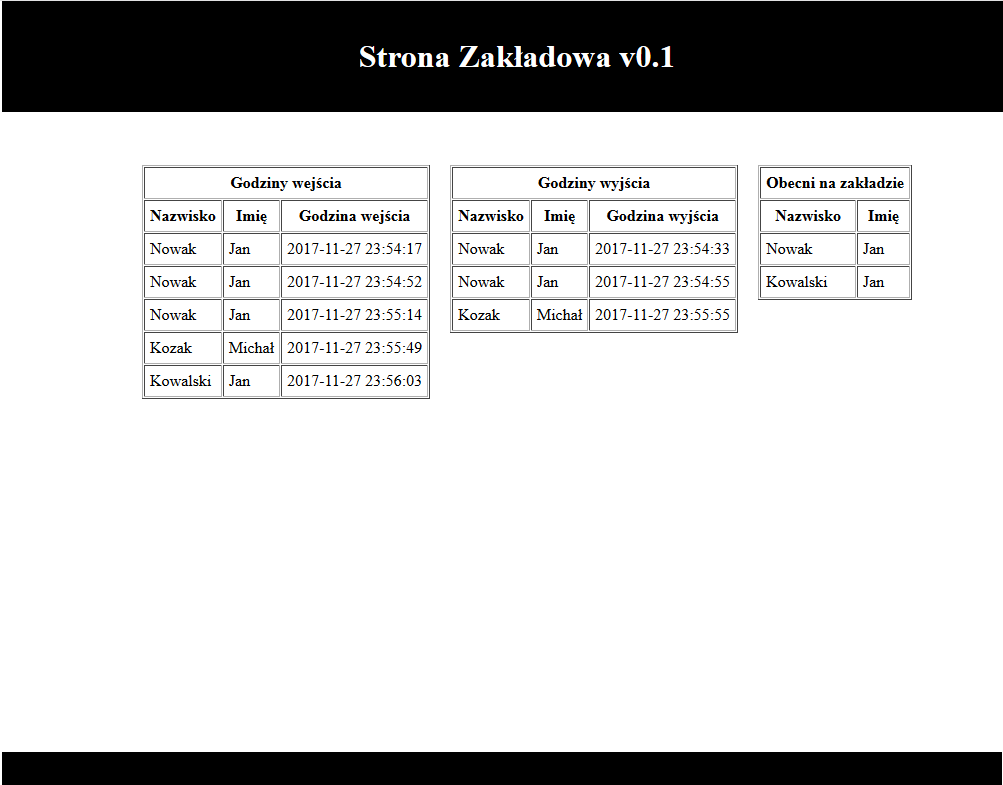
\includegraphics[width=260px]{obrazy/strona.png}}
\end{figure}

Dane przedstawione na stronie pochodziły z bazy danych, która otrzymywała dane za każdym razem, gdy pracownik przykładał kartę do czytnika RFID. Buzzer oraz diody LED  zaimplementowane w systemie informowały czy dane pracownika zostały poprawnie odczytane  poprzez zgaszenie  zielonej diody i zaświecenie się czerwonej diody, czemu towarzyszył pojedynczy dźwięk. Następnie po około 3 sekundach urządzenie sygnalizowało gotowość do kolejnego odczytu poprzez podwójny dźwięk i przywrócenie pierwotnego stanu diod. W tym momencie kolejny pracownik mógł już przyłożyć swoją kartę do czytnika a na stronie pojawiały się odpowiednie zmiany.

\section{Sprint 2}

\subsection{Cel} Celem drugiego sprintu jest rozbudowa strony internetowej zakładu o takie funkcje jak: logowanie, funkcję dodawania i usuwania pracowników oraz możliwość obliczania przepracowanego przez nich czasu. W efekcie dostęp do strony zostanie zabezpieczony przed nieuprawnionymi osobami a kadrowy i księgowy zyskają nowe narzędzia ułatwiające ich pracę. Ten pierwszy uzyska kontrolę nad zmianami liczebności załogi zakładu, natomiast ten drugi będzie mógł w łatwy sposób dokonywać co miesięcznych zestawień przepracowanych godzin przez zatrudnione osoby. Ponadto dodana zostanie funkcja ułatwiająca dodawanie nowych kart pracowniczych do bazy danych w ten sposób, iż nie trzeba będzie ręcznie wprowadzać numeru ID karty do bazy, ale wystarczy samo jej przyłożenie do czytnika RFID a program automatycznie wykona powyższą operację.

\subsection{Sprint Planning/Backlog}

\paragraph{Tytuł zadania.} Podsumowanie przepracowanych godzin.
\begin{itemize}
\item Estymata: Large przy użyciu skali rozmiarów T-shirtów (10 osobogodzin).
\end{itemize}

\paragraph{Tytuł zadania.} Logowanie do strony zakładowej.
\begin{itemize}
\item Estymata: Medium przy użyciu skali rozmiarów T-shirtów (5 osobogodzin).
\end{itemize}

\paragraph{Tytuł zadania.} Dodawanie oraz usuwanie nowych pracowników.
\begin{itemize}
\item Estymata: Medium przy użyciu skali rozmiarów T-shirtów (5 osobogodzin).
\end{itemize}

\paragraph{Tytuł zadania.} Dodawanie nowych kart do bazy danych.
\begin{itemize}
\item Estymata: Medium przy użyciu skali rozmiarów T-shirtów (6 osobogodzin).
\end{itemize}



\subsection{Realizacja}

\paragraph{Tytuł zadania.} Podsumowanie przepracowanych godzin.
\subparagraph{Wykonawca.} Łukasz Horowski, Mateusz Morawa.
\subparagraph{Realizacja.} W celu realizacji powyższego zadania została stworzona nowa zakładka w menu strony zakładowej zawierająca kod wykonany w języku PHP. Po jej kliknięciu następuje sprawdzenie, kiedy miało miejsce ostatnie podsumowanie przepracowanych godzin oraz wyświetlenie daty tego zestawienia. Jeśli operacja ta odbyła się w innym miesiącu niż obecny to pojawia się możliwość zainicjowania nowego podsumowania poprzez naciśnięcie przycisku "Podsumuj". Wtedy uruchomiona zostaje pętla sprawdzająca i wyświetlająca czas pracy każdego pracownika, znajdującego się w bazie danych, w poszczególnych dniach miesiąca. Otrzymane w ten sposób wartości są zaokrąglane poprzez funkcję floor w celu uzyskania pełnych godzin spędzonych na zakładzie. Po zakończeniu wykonywania się pętli zostaje wyświetlona tabela podsumowująca ilość godzin przepracowanych przez każdego pracownika w danym miesiącu. Powyższe zadanie było jak dotąd najtrudniejsze ze wszystkich do wykonania - w szczególności kwestia obliczania czasu pracy pracownika, który w ciągu dnia kilkakrotnie przychodził i opuszczał zakład, sprawiła najwięcej problemów.
Kod programu wyświetlający miesięczne podsumowanie godzin przepracowanych przez zatrudnione osoby (środowisko \texttt{verbatim}): \begin{verbatim}
for($i=0;$i<=$liczbapracownikow-1;$i++){
   for ($j=0;$j<=3;$j++){
       switch($j){
          case 0:
             echo "Pracownik : ";
             break;
          case 1:
             echo " WE : ";
             break;
          case 2:
             echo " WY : ";
             break;	
          case 3:
             echo " Godziny: ";
             break;
       }
       echo $podsum[$i][$j];
   }
   echo "</BR>";
}
\end{verbatim}

\paragraph{Tytuł zadania.} Logowanie do strony zakładowej.
\subparagraph{Wykonawca.} Łukasz Horowski, Bartłomiej Kmak, Grzegorz Jasiński, Łukasz Mirek.
\subparagraph{Realizacja.} W języku PHP został napisany fragment kodu uzupełniający stronę zakładową, odpowiadający za logowanie się użytkowników. Został on napisany w edytorze tekstu Notepad++, który pozwala na sprawną modyfikację kodu oraz kontrolę składni wybranego języka. Po wejściu na stronę wyświetla się formularz z miejscem na wpisanie loginu użytkownika oraz hasła. Na stronę będą mogli się zalogować kierownik, księgowy, kadrowy oraz pracownicy dodani do bazy MySQL. Pracownik, który wejdzie na stronę i będzie chciał się zalogować musi wpisać login oraz hasło. Fragment kodu przedstawionego poniżej programu sprawdzi w bazie czy istnieje pracownik z podanym loginem oraz czy podane hasło odpowiada zaszyfrowanemu hasłu w bazie danych. Jeśli login i hasło zostaną podane poprawnie, pracownik otrzyma dostęp do zawartości strony zakładowej i odpowiednich funkcji stosownych do jego stanowiska. W razie podania błędnych danych do logowania, zostaną wyświetlone odpowiednie komunikaty: dla błędnego loginu "Nie istnieje takie konto użytkownika!" lub dla błędnego hasła "Podane hasło jest nieprawidłowe!". 
Kod programu (środowisko \texttt{verbatim}): 
\begin{verbatim}
if(!empty($_POST)){
	if (!empty($_POST['login']) && (!empty($_POST['password']))){
		$login=$_POST['login'];
		$password=$_POST['password'];
		//sprawdzenie poprawności
		$dane = mysqli_query($db , "SELECT * FROM websiteusers 
		WHERE Login='$login' LIMIT 1");
		if (mysqli_num_rows($dane)===1){
			$dane=mysqli_fetch_assoc($dane);
			if (md5($password)===$dane['Haslo']){
                //logowanie i pobranie sesji
				$_SESSION['id'] = $dane['Id'];
				header("Location: ?a=start");
			}
			else {
				echo '<CENTER>Podane hasło jest nieprawidłowe!</CENTER><BR>';
			}
		}
		else {
			echo '<CENTER>Nie istnieje takie konto użytkownika!</CENTER><BR>';
		}		
	}else {
		echo '<CENTER>Uzupełnij wszystkie dane!</CENTER><BR>';
	}
};
\end{verbatim}

\paragraph{Tytuł zadania.} Dodawanie oraz usuwanie pracowników.
\subparagraph{Wykonawca.} Łukasz Horowski, Bartłomiej Kmak, Grzegorz Jasiński, Łukasz Mirek.
\subparagraph{Realizacja.} W języku PHP został napisany skrypt i umieszczony na stronie zakładowej w odpowiedniej zakładce menu, odpowiadający za dodanie do bazy danych pracownika za pomocą zamieszczonego formularza. Podczas tej operacji kierownik bądź kadrowy, po uzupełnieniu danych osobowych nowego pracownika, będzie tworzył dla niego konto umożliwiające logowanie na stronę zakładową z odpowiednim loginem oraz hasłem. Za usuwanie pracownika odpowiada osobny skrypt znajdujący się w osobnej zakładce menu. Dzięki niemu kierownik bądź kadrowy po znalezieniu na liście pracowników osoby do zwolnienia wpisuje jej ID w formularzu i poprzez kliknięcie na przycisk dokonuje jej usunięcia z bazy danych.
Kod programu odpowiedzialny za dodawanie pracownika. (środowisko \texttt{verbatim}): 
\begin{verbatim}
<?php
if(!empty($_POST)){
if (empty($_POST['login']) || empty($_POST['password'])
|| empty($_POST['email']))
echo '<CENTER>Uzupełnij wszystkie pola!</CENTER><BR>';
else
	{
	$connection	= new mysqli("localhost","root", "" ,"zpi");
	$login = ($_POST['login']);
	$password = ($_POST['password']);
	$email = ($_POST['email']);
	$idkarty = $_POST['idkarty'];
	
	$idstanowiska =	($_POST['idstanowiska']);
	$nazwisko = $_POST['nazwisko'];
	$imie = $_POST['imie'];
	$datazatrudnienia =	$_POST['datazatrudnienia'];
	$miejscowosc = $_POST['miejscowosc'];
	$ulica	= $_POST['ulica'];
	$nrdomu	= $_POST['nrdomu'];
	$nrmieszkania = $_POST['nrmieszkania'];
	$kodpocztowy = $_POST['kodpocztowy'];
	$stawka	=	$_POST['stawka'];
	$connection->query("SELECT * FROM stanowisko WHERE id =$idstanowiska");
	$connection->query("SELECT * FROM karty WHERE id =$idkarty");
	//sprawdzanie poprawności znaków
	if (! ctype_alnum($login) ) 
	echo '<CENTER>Wprowadzono nieprawidłową nazwę 
	użytkownika!</CENTER><BR>';
	else if (! filter_var($email,FILTER_VALIDATE_EMAIL) ) 
	echo '<CENTER>Wprowadzono 
	nieprawidłowy adres email!</CENTER><BR>!';
	else{ 

		// sprawdzanie czy dane istnieją
		$login2 = ($connection->query("SELECT Login FROM websiteusers 
		WHERE Login='$login' "));
		$login2 = mysqli_fetch_assoc($login2);
		$email2 = ($connection->query("SELECT Email FROM websiteusers 
		WHERE Email='$email' "));
		$email2 = mysqli_fetch_assoc($email2);
		//warunki jeżeli zajęty login lub email
		if (($login2['Login'])!='') echo '<CENTER>Nazwa użytkownika 
		jest już zajęta!</CENTER><BR>';
		elseif (($email2['Email'])!='') echo '<CENTER>Wprowadzony 
		adres E-mail jest już zajęty!</CENTER><BR>';
		else{
			// zakladanie konta
			$password = md5($password);
			$connection->query("INSERT INTO users (Login,Password,Email) 
			VALUES ('$login','$password','$email')");
			$connection->query("INSERT INTO pracownicy (IdKarty, Nazwisko, 
			Imie, Miejscowosc, Ulica, NrDomu, NrMieszkania, KodPocztowy, Stawka)
			VALUES ('$idkarty', '$nazwisko', '$imie', '$miejscowosc', '$ulica',
			 '$nrdomu', '$nrmieszkania', '$kodpocztowy', '$stawka');");
			echo "<CENTER>Konto zostało pomyślnie założone!</CENTER>";
		}
	}
}
};
?>
\end{verbatim}
Kod programu odpowiedzialny za usuwanie pracownika. (środowisko \texttt{verbatim}): 
\begin{verbatim}
if ( $id > 1){ 
		$zapytanie="DELETE from RejestrWe WHERE IdPracownika='$id'"; 
		$wykonaj = mysqli_query($db,$zapytanie);
		$zapytanie="DELETE from RejestrWy WHERE IdPracownika='$id'"; 
		$wykonaj = mysqli_query($db,$zapytanie);
		$zapytanie="DELETE from WebSiteUsers WHERE IdPracownika='$id'"; 
		$wykonaj = mysqli_query($db,$zapytanie);
		$zapytanie="DELETE from ZestawienieDzienne WHERE IdPracownika='$id'"; 
		$wykonaj = mysqli_query($db,$zapytanie);
		$zapytanie="DELETE from ZestawienieMiesieczne WHERE IdPracownika='$id'"; 
		$wykonaj = mysqli_query($db,$zapytanie);
		$zapytanie="DELETE from Pracownicy WHERE Id='$id'"; 
		$wykonaj = mysqli_query($db,$zapytanie);
	}
	else{
		echo "Nie można zwolnić głównego kierownika!";
	}
}
\end{verbatim}

\paragraph{Tytuł zadania.} Dodawanie nowych kart do bazy danych.
\subparagraph{Wykonawca.} Łukasz Horowski, Mateusz Morawa.
\subparagraph{Realizacja.} W języku Python został utworzony program, który za pomocą czytnika RFID odczytuje numery ID kart i dodaje je do bazy danych (tabela Karty). Program ten sprawdza czy odczytane ID istnieje już w tej tabeli czy też nie i wydaje odpowiednie sygnały buzzerem oraz diodami LED. Jeśli ID nie istnieje, zapala się zielona dioda i wydawany jest jeden dłuższy sygnał a po 3 sekundach 2 krótsze, wtedy numer ID jest dopisywany do bazy. W przeciwnym wypadku nadal pali się czerwona dioda a buzzer wydaje 5x krótki sygnał.
Kod programu ilustrujący procedurę dodawania nowej karty do bazy danych oraz towarzyszące temu sygnały świetlne i dźwiękowe. (środowisko \texttt{verbatim}): 
\begin{verbatim}
if (uid == "None"):
    db.execute("INSERT INTO Karty(IdKarty) VALUES ("+idkarty+");")
    connect.commit()
    print "Dodano nową kartę"
    GPIO.output(11, 0)
    GPIO.output(12, 1)
    GPIO.output(13, 1)
    time.sleep(0.5)
    GPIO.output(13, 0)
    time.sleep(2)
    GPIO.output(13, 1)
    time.sleep(0.2)
    GPIO.output(13, 0)
    time.sleep(0.2)
    GPIO.output(13, 1)
    time.sleep(0.2)
    GPIO.output(13, 0)
\end{verbatim}


\subsection{Sprint Review/Demo}
Dnia 20.12.17 r. przedstawiono demo produktu w ramach drugiego Sprintu. Wszystkie założone cele zawarte w backlog itemach zaplanowanych na ten sprint zostały zrealizowane bez żadnych przeszkód. Prezentacja sprintu zawierała przedstawienie możliwości zalogowania się na stronę zakładową, z czym wiązał się różny dostęp do funkcji w zależności od uprawnień zalogowanego użytkownika. Przykładowo kierownik, który dysponuje pełnymi prawami może zatrudniać, zwalniać pracowników oraz kontrolować podsumowania miesięczne przepracowanych godzin przez pracowników. Natomiast pracownik po zalogowaniu może jedynie sprawdzić kto jest obecnie na zakładzie. Ponadto została zaprezentowana funkcja dodawania do bazy danych nowych kart dla pracowników. Po przyłożeniu karty, która nie była dodana do bazy danych, buzzer wydał dźwięk i karta została dopisana do kart pustych. Kiedy ta sama karta została przyłożona ponownie, wyświetlił się komunikat, że karta jest już dodana do bazy. Jako ostatnia została zaprezentowana funkcja dodawania i usuwania nowych pracowników. Ta pierwsza operacja odbyła się poprzez wypełnienie formularza, gdzie była możliwość wyboru stanowiska oraz pustej karty z rozwijanej listy, pola z danymi osobowymi oraz miejsce wpisania loginu oraz hasła przyszłego pracownika, który będzie mógł się logować na stronie. Zakończyła się ona całkowitym sukcesem podobnie jak test zwalniania pracownika, co odbyło się poprzez podanie ID pracownika w odpowiedniej rubryce formularza. Warto wspomnieć, iż dla ułatwienia odszukania ID pracownika, wszyscy zatrudnieni są wyświetleni w tabeli poniżej formularza. Zwolnienie głównego kierownika jest zablokowane.


\section{Sprint 3}

\subsection{Cel} Celem trzeciego sprintu jest dalsza rozbudowa strony zakładowej. Kierownik otrzyma uprawnienia do wszystkich funkcji dostępnych na stronie, dzięki czemu podczas nieobecności któregoś z pracowników będzie mógł wykonać interesujące go zmiany. Kolejną wprowadzoną modyfikacją będzie możliwość przywrócenia hasła w razie jego zapomnienia. Odbywać się to będzie poprzez serwer poczty elektronicznej (MTA) o nazwie SSMTP  zainstalowany na serwerze. Wysyłał on będzie wiadomość z nowym hasłem na adres e-mail danej osoby, dzięki czemu będzie ona mogła odzyskać do niej dostęp. Ostatnim zadaniem zrealizowanym w tym sprincie będzie dodanie funkcji obliczającej wynagrodzenia pracowników. Wynagrodzenie będzie wyliczane na podstawie pełnych przepracowanych godzin oraz stawki pracownika zawartej w umowie w przedziale czasowym od ósmej do szesnastej czyli w godzinach pracy zakładu. 

\subsection{Sprint Planning/Backlog}

\paragraph{Tytuł zadania.} Obliczanie wynagrodzenia.
\begin{itemize}
\item Estymata: Large przy użyciu skali rozmiarów T-shirtów (10 osobogodzin).
\end{itemize}

\paragraph{Tytuł zadania.} Przywracanie hasła.
\begin{itemize}
\item Estymata: Large przy użyciu skali rozmiarów T-shirtów (10 osobogodzin).
\end{itemize}

\paragraph{Tytuł zadania.} Uprawnienia kierownika do wszystkich funkcji.
\begin{itemize}
\item Estymata: Small przy użyciu skali rozmiarów T-shirtów (2 osobogodzin).
\end{itemize}


\subsection{Realizacja}

\paragraph{Tytuł zadania.} Obliczanie wynagrodzenia.
\subparagraph{Wykonawca.} Łukasz Horowski, Bartłomiej Kmak, Grzegorz Jasiński, Łukasz Mirek.
\subparagraph{Realizacja.}  W celu realizacji zadania została stworzona nowa zakładka w menu strony zakładowej, która pojawia się gdy rozpocznie się nowy miesiąc. Po kliknięciu w nią automatycznie tworzone jest podsumowanie oraz zostaje obliczone wynagrodzenie zgodnie ze stawką godzinową w umowie. Skrypt w tym pliku jest niemal identyczny jak w pliku z podsumowaniem, lecz tutaj nie mamy wyboru, co chcemy podsumować, lecz automatycznie podsumowywany jest ostatni miesiąc. Po podliczeniu dane są wpisywane do bazy danych a zakładka jest nieaktywna do rozpoczęcia kolejnego miesiąca. Dodatkowo została zmodyfikowana zakładka podsumowania, tak aby można było sprawdzić tam statystyki w obecnym miesiącu.

\paragraph{Tytuł zadania.} Przywracanie hasła.
\subparagraph{Wykonawca.} Mateusz Morawa, Łukasz Horowski.
\subparagraph{Realizacja.} Pierwszym krokiem niezbędnym do wykonania zadania było zainstalowanie na Raspberry Pi serwera poczty elektronicznej (MTA) o nazwie SSMTP oraz zbioru narzędzi do obsługi poczty - pakiet mailutils. Odbyło się to poprzez użycie polecenia: 
\begin{verbatim} sudo apt-get install ssmtp mailutils\end{verbatim} 
Następnie koniecznym było dokonanie edycji pliku konfiguracyjnego ssmtp.conf, w którym ustawione zostały dane logowania do serwera IMAP oraz odpowiedni poziom zabezpieczeń. W celu przetestowania działania serwera poczty elektronicznej stworzone zostały przykładowe konta pocztowe na zewnętrznym serwisie webmail, na które rozesłane zostały testowe e-maile. Kiedy ten etap zakończył się sukcesem utworzony został skrypt w języku PHP, który po kliknięciu na link: "Odzyskaj hasło" i podaniu loginu oraz adresu e-mail wysyła wiadomość z nowym hasłem dla danego pracownika. Wtedy może on za jego pomocą zalogować się na swoje konto, tym samym ponownie uzyskując dostęp do funkcjonalności strony internetowej. Kod skryptu PHP odpowiedzialny za wysyłanie e-maila (środowisko \texttt{verbatim}):
\begin{verbatim}
$to = $email;
$subject = "Odzyskiwanie konta do strony zakladowej";
$message = "Nowe hasło do strony zakładowej: ".$nowehaslo;
$from = "konto.zakladu@gmail.pl";
$headers = "From:".$from;
mail($to,$subject,$message,$headers);
$md5haslo = md5($nowehaslo);
mysqli_query($db ,"UPDATE `WebSiteUsers` SET Haslo = '".$md5haslo."' 
WHERE Login='".$login."';");
echo "<CENTER>Wysłano nowe hasło na podany adres email.</BR>
\end{verbatim}

\paragraph{Tytuł zadania.} Uprawnienia kierownika do wszystkich funkcji.
\subparagraph{Wykonawca.} Łukasz Horowski, Bartłomiej Kmak, Grzegorz Jasiński, Łukasz Mirek.
\subparagraph{Realizacja.}  Do realizacji powyższego zadania użyliśmy instrukcji warunkowej IF. Sprawdzamy w niej czy idstanowiska zalogowanej osoby (1 - kierownik, 2 - księgowy, 3 - kadrowy, 4 - pracownik) zgadza się z zapisem w warunku. Przykładowo poniższy kod przydziela kierownikowi pełne prawa do zarządzania na stronie: 
\begin{verbatim}
if ($idstanowiska == 1){
		$ostatnie = mysqli_fetch_array(mysqli_query($db, "SELECT * FROM
		ZestawienieMiesieczne ORDER BY id DESC LIMIT 1"));
		$data = $ostatnie['DataPodsumowania'];
		$data = strtotime( $data );
		if (date('m-Y',$data)!=date('m-Y')){		
			echo "<a href='?a=wynagrodzenie' >! Wynagrodzenie !</a><BR><BR>";
		}
		echo "<a href='?a=zatrudnij'>Zatrudnij pracownika</a><BR><BR>";
		echo "<a href='?a=zwolnij'>Zwolnij pracownika</a><BR><BR>";
	}
\end{verbatim}
Natomiast logujący się pracownik z idstanowiska równym 4 posiada tylko prawo do sprawdzenia, kto aktualnie jest na zakładzie oraz wyświetlenia podsumowania za aktualny miesiąc. 


\subsection{Sprint Review/Demo}
W dniu 10.01.2018 r. zostało przedstawione demo sprintu nr 3. Celem tego sprintu było uzupełnienie strony zakładowej o nowe funkcje tj:
\begin{itemize}
	\item pełne prawa Kierownika na stronie,
	\item obliczanie wynagrodzenia za poprzedni miesiąc,
	\item odzyskiwanie hasła dla każdego użytkownika strony.
\end{itemize}
Wszystkie założone zadania na ten sprint zostały zrealizowane. Kierownikowi zostały przypisane wszystkie prawa i ma on dostęp do wszystkich funkcji zamieszczonych na stronie.
Do realizacji zadania z odzyskiwaniem hasła konieczne było zainstalowanie serwera poczty SSMTP. Użytkownik chcąc odzyskać hasło musi podać login oraz adres e-mail istniejący w bazie systemowej. W przypadku podania błędnych danych wyświetli się komunikat: "Podano nieprawidłowy adres e-mail bądź login". Wiadomość z nowo wygenerowanym hasłem przychodzi na podany prawidłowy adres e-mail, dzięki czemu użytkownik może bez problemu zalogować się na stronie.
Obliczanie wynagrodzenia odbywa się przez zliczenie przepracowanych przez pracownika godzin  oraz pomnożenie ich przez stawkę. Można to wykonać tylko po zakończonym pełnym miesiącu.

\section{Sprint 4}

\subsection{Cel} W ramach ostatniego sprintu udostępniona zostanie funkcja drukowania do pliku w formacie PDF zestawienia miesięcznego wynagrodzenia każdego z pracowników. Dzięki temu możliwe będzie zarchiwizowanie dokumentacji płacowej na potrzeby kontroli urzędowej oraz analizy statystycznej. Ponadto wykonana zostanie modernizacja funkcji podsumowania wynagrodzenia o wyświetlenie zestawienia z każdego miesiąca w roku, co pozwoli pracownikowi na sprawdzenie swoich wcześniejszych zarobków. Na końcu zostaną przeprowadzone finalne testy całego systemu w celu wykrycia i poprawienia ewentualnych błędów.  

\subsection{Sprint Planning/Backlog}

\paragraph{Tytuł zadania.} Drukowanie do pliku PDF zestawienia miesięcznego wynagrodzenia pracowników.
\begin{itemize}
	\item Estymata: Medium przy użyciu skali rozmiarów T-shirtów (5 osobogodzin).
\end{itemize}

\paragraph{Tytuł zadania.} Funkcja umożliwiająca pracownikowi sprawdzenie wynagrodzenia (opcjonalna).
\begin{itemize}
	\item Estymata: Small przy użyciu skali rozmiarów T-shirtów (2 osobogodzin).
\end{itemize}

\paragraph{Tytuł zadania.} Finalne testy całego systemu.
\begin{itemize}
	\item Estymata: Large przy użyciu skali rozmiarów T-shirtów (15 osobogodzin).
\end{itemize}

\subsection{Realizacja}

\paragraph{Tytuł zadania.} Drukowanie do pliku PDF zestawienia miesięcznego wynagrodzenia pracowników.
\subparagraph{Wykonawca.} Mateusz Morawa, Łukasz Horowski.
\subparagraph{Realizacja.} Zadanie, polegające na umożliwieniu księgowemu wykonania wydruku zestawienia miesięcznego wynagrodzenia pracowników do pliku PDF, wymagało napisania skryptu PHP i umieszczenia go na stronie w zakładce Wynagrodzenia. Do jego poprawnego działania konieczne było użycie klasy FPDF, dostępnej na wolnej licencji wraz z plikami czcionki Arial, zawierającej polskie znaki \cite{FDPF}. Skrypt ten jest wywoływany po kliknięciu na przycisk "Drukuj", co powoduje utworzenie pliku PDF i wysłanie go do przeglądarki w celu zapisania go na dysku twardym. W pliku tym znajduje się tabela z danymi pracowników oraz ich wynagrodzeniami za dany miesiąc. Kod programu odpowiedzialny za wygenerowanie pliku PDF (środowisko \texttt{verbatim}): \begin{verbatim}
require('fpdf/fpdf.php');
$pdf = new PDF();
$pdf->AddFont('arial_ce','','arial_ce.php');
$pdf->SetFont('arial_ce','',14);
$pdf->AddPage();
$pdf->Ln();
$opis=iconv('UTF-8','windows-1250//TRANSLIT',
'Zestawienie miesięczne wynagrodzenia za: ');
$headerUTF = array('Imię i nazwisko', 'Wynagrodzenie (w zł)');
$pdf->Cell(10,10, $opis.date('m-Y'));
$pdf->Ln();
$pdf->Table($header,$data);
\end{verbatim}

\paragraph{Tytuł zadania.} Funkcja umożliwiająca pracownikowi sprawdzenie wynagrodzenia (opcjonalna).
\subparagraph{Wykonawca.} Łukasz Mirek, Grzegorz Jasiński, Bartłomiej Kmak.
\subparagraph{Realizacja.} W ramach realizacji tego zadania, w głównej mierze została wykorzystana poprzednia funkcja obliczania wynagrodzenia, gdyż obie funkcje działają na podobnej zasadzie. Plik odpowiadający za funkcję wynagrodzenia został skopiowany i odpowiednio zmodyfikowany aby wyświetlał tylko dane (bez aktualizacji ich do bazy), tak aby można było wybrać sobie w nim konkretny miesiąc, w tym także obecny. Dodatkowo została utworzona w nim odpowiednia funkcja sprawdzająca na jakim stanowisku został zalogowany użytkownik: jeśli zalogowano jako pracownik dane, które są wyświetlane tyczą się tylko tego pracownika, jeżeli zaś zalogowano się na którymkolwiek stanowisku administracyjnym wtedy dane są wyświetlane dla każdego pracownika firmy.   
 

\paragraph{Tytuł zadania.} Finalne testy całego systemu.
\subparagraph{Wykonawca.} Mateusz Morawa, Łukasz Horowski, Łukasz Mirek, Grzegorz Jasiński, Bartłomiej Kmak.
\subparagraph{Realizacja.} 
W celu sprawdzenia poprawności działania całego systemu, przeprowadziliśmy finalne testy wszystkich komponentów działających w systemie. W pierwszej kolejności przetestowaliśmy połączenie modułu RFID z urządzeniem Raspberry Pi. Schemat połączeniowy został wykonany zgodnie z wcześniejszymi założeniami. Całość działa poprawnie. Następnie rozpoczęliśmy testy działania elementów strony internetowej, pierwszym testem było sprawdzenie poprawności skryptu odpowiadającego za logowanie się pracowników. W tym celu utworzyliśmy kilku przykładowych pracowników w bazie danych i przeprowadziliśmy próby logowania się na ich konta. Wraz z tworzeniem kont sprawdzona została poprawność działania systemu bazodanowego, który odpowiada za przechowywanie danych pracowników i firmy.

Na wcześniej utworzonych kontach pracowników skorzystaliśmy z funkcji przywrócenia hasła w celu jej weryfikacji. Na podany adres e-mail pracownika, który był wymagany podczas rejestracji, otrzymaliśmy wiadomość z nowo wygenerowanym hasłem. E-mail z nowym hasłem został wysłany do pracownika po wcześniejszej weryfikacji i sprawdzeniu poprawności adresu e-mail i loginu pracownika. Cała procedura przebiegła pomyślnie a za pomocą nowego hasła pracownik ponownie mógł zalogować się na stronę zakładową.

Kolejnym elementem który przetestowaliśmy był system rejestracji wejść i wyjść pracowników oraz wyświetlanie tych informacji w tabeli. W tym celu musieliśmy skorzystać z kart, które wcześniej przypisaliśmy do testowego konta. Po przyłożeniu karty do czytnika, wydawał on pojedynczy dźwięk oraz sygnalizował wejście zapalającą się zieloną diodą. Po około 3 sekundach można było przyłożyć ponownie kartę, aby sczytać godzinę. System poprawnie wykrywa czy dany pracownik który przykłada kartę, próbuje wyjść, czy dopiero ma zamiar zarejestrować wejście na zakład. Wszystkie te dane zostają przekazane do bazy danych, z której na stronie internetowej tworzy się oraz wyświetla tabela z wejściami, wyjściami pracowników oraz osobami, które znajdują się aktualnie na zakładzie. Po dokładnym przetestowaniu tej funkcjonalności stwierdziliśmy, że działa ona poprawnie.

Przetestowaliśmy również opcję dodawania oraz usuwania pracowników. W jednej z zakładek znajduje się formularz, w którym wybieramy stanowisko, nr karty (pracownik może zostać dodany tylko jeżeli istnieje wolna karta) oraz uzupełniamy dane osobowe pracownika. Przy dodawaniu użytkownika wszystkie pola muszą zostać uzupełnione, w razie braku którejś informacji system poinformuje o błędzie w formularzu. Uzupełniając dane do logowania, w polu adres e-mail musi występować poprawna składnia adresu, w przeciwnym wypadku nie stworzymy konta. Po utworzeniu konta na stronie, sprawdziliśmy czy zostało ono poprawnie dodane do bazy. Naszym testom została poddana również funkcja usuwania pracowników. Działa ona prawidłowo. Po usunięciu pracownika na stronie, usuwa się on również z bazy danych. Zostało przetestowane zabezpieczenie uniemożliwiające usunięcie głównego kierownika zakładu, który posiada uprawnienia administratora.
Każdy z pracowników posiada odpowiednie uprawnienia, co do stanowiska jakie obejmuje. Sprawdziliśmy to przez zalogowanie się na konta użytkowników należących do każdej z grupy uprawnień tj. kierownik, kadrowy, księgowy oraz pracownik.


\subsection{Sprint Review/Demo}
Dnia 24.01.18 odbył się ostatni sprint rewiev. Została na nim zaprezentowana finalna, w pełni funkcjonalna wersja systemu. Wszystkie założenia zostały wykonane w wyznaczonych terminach. W porównaniu do poprzedniej wersji dodane zostały następujące funkcję:
\begin{itemize}
\item funkcja wydruku zestawienia miesięcznego,
\item zmiana hasła użytkownika,
\item poprawki interfejsu oraz bazy danych.
\end{itemize}


\begin{thebibliography}{9}

\bibitem{Cov} S. R. Covey, {\em 7 nawyków skutecznego działania}, Rebis, Poznań, 2007.

\bibitem{Oet} Tobias Oetiker i wsp., Nie za krótkie wprowadzenie do systemu \LaTeX  \ $2_\varepsilon$, \url{ftp://ftp.gust.org.pl/TeX/info/lshort/polish/lshort2e.pdf}

\bibitem{SchSut} K. Schwaber, J. Sutherland, {\em Scrum Guide}, \url{http://www.scrumguides.org/}, 2016.

\bibitem{FDPF} Biblioteka FPDF do PHP i polskie znaki \url{http://ntxt.net/?id=polskie_znaki_w_FPDF}

\bibitem{Rasp} Raspberry Pi 3 Model B \& MIFARE RC522 RFID Tag Reading \\ \url{http://www.instructables.com/id/Raspberry-Pi-3-Model-B-MIFARE-RC522-RFID-Tag-Readi/}

\bibitem{apr} \url{https://agilepainrelief.com/notesfromatooluser/tag/scrum-by-example}

\bibitem{us} \url{https://www.tutorialspoint.com/scrum/scrum_user_stories.htm}

\end{thebibliography}

\end{document}

% ----------------------------------------------------------------
